\documentclass[10pt]{article}
\pdfinfoomitdate=1
\pdftrailerid{}
\usepackage{tmlr}

%%%%% NEW MATH DEFINITIONS %%%%%

\usepackage{amsmath,amsfonts,bm}

% Mark sections of captions for referring to divisions of figures
\newcommand{\figleft}{{\em (Left)}}
\newcommand{\figcenter}{{\em (Center)}}
\newcommand{\figright}{{\em (Right)}}
\newcommand{\figtop}{{\em (Top)}}
\newcommand{\figbottom}{{\em (Bottom)}}
\newcommand{\captiona}{{\em (a)}}
\newcommand{\captionb}{{\em (b)}}
\newcommand{\captionc}{{\em (c)}}
\newcommand{\captiond}{{\em (d)}}

% Highlight a newly defined term
\newcommand{\newterm}[1]{{\bf #1}}


% Figure reference, lower-case.
\def\figref#1{figure~\ref{#1}}
% Figure reference, capital. For start of sentence
\def\Figref#1{Figure~\ref{#1}}
\def\twofigref#1#2{figures \ref{#1} and \ref{#2}}
\def\quadfigref#1#2#3#4{figures \ref{#1}, \ref{#2}, \ref{#3} and \ref{#4}}
% Section reference, lower-case.
\def\secref#1{section~\ref{#1}}
% Section reference, capital.
\def\Secref#1{Section~\ref{#1}}
% Reference to two sections.
\def\twosecrefs#1#2{sections \ref{#1} and \ref{#2}}
% Reference to three sections.
\def\secrefs#1#2#3{sections \ref{#1}, \ref{#2} and \ref{#3}}
% Reference to an equation, lower-case.
\def\eqref#1{equation~\ref{#1}}
% Reference to an equation, upper case
\def\Eqref#1{Equation~\ref{#1}}
% A raw reference to an equation---avoid using if possible
\def\plaineqref#1{\ref{#1}}
% Reference to a chapter, lower-case.
\def\chapref#1{chapter~\ref{#1}}
% Reference to an equation, upper case.
\def\Chapref#1{Chapter~\ref{#1}}
% Reference to a range of chapters
\def\rangechapref#1#2{chapters\ref{#1}--\ref{#2}}
% Reference to an algorithm, lower-case.
\def\algref#1{algorithm~\ref{#1}}
% Reference to an algorithm, upper case.
\def\Algref#1{Algorithm~\ref{#1}}
\def\twoalgref#1#2{algorithms \ref{#1} and \ref{#2}}
\def\Twoalgref#1#2{Algorithms \ref{#1} and \ref{#2}}
% Reference to a part, lower case
\def\partref#1{part~\ref{#1}}
% Reference to a part, upper case
\def\Partref#1{Part~\ref{#1}}
\def\twopartref#1#2{parts \ref{#1} and \ref{#2}}

\def\ceil#1{\lceil #1 \rceil}
\def\floor#1{\lfloor #1 \rfloor}
\def\1{\bm{1}}
\newcommand{\train}{\mathcal{D}}
\newcommand{\valid}{\mathcal{D_{\mathrm{valid}}}}
\newcommand{\test}{\mathcal{D_{\mathrm{test}}}}

\def\eps{{\epsilon}}


% Random variables
\def\reta{{\textnormal{$\eta$}}}
\def\ra{{\textnormal{a}}}
\def\rb{{\textnormal{b}}}
\def\rc{{\textnormal{c}}}
\def\rd{{\textnormal{d}}}
\def\re{{\textnormal{e}}}
\def\rf{{\textnormal{f}}}
\def\rg{{\textnormal{g}}}
\def\rh{{\textnormal{h}}}
\def\ri{{\textnormal{i}}}
\def\rj{{\textnormal{j}}}
\def\rk{{\textnormal{k}}}
\def\rl{{\textnormal{l}}}
% rm is already a command, just don't name any random variables m
\def\rn{{\textnormal{n}}}
\def\ro{{\textnormal{o}}}
\def\rp{{\textnormal{p}}}
\def\rq{{\textnormal{q}}}
\def\rr{{\textnormal{r}}}
\def\rs{{\textnormal{s}}}
\def\rt{{\textnormal{t}}}
\def\ru{{\textnormal{u}}}
\def\rv{{\textnormal{v}}}
\def\rw{{\textnormal{w}}}
\def\rx{{\textnormal{x}}}
\def\ry{{\textnormal{y}}}
\def\rz{{\textnormal{z}}}

% Random vectors
\def\rvepsilon{{\mathbf{\epsilon}}}
\def\rvtheta{{\mathbf{\theta}}}
\def\rva{{\mathbf{a}}}
\def\rvb{{\mathbf{b}}}
\def\rvc{{\mathbf{c}}}
\def\rvd{{\mathbf{d}}}
\def\rve{{\mathbf{e}}}
\def\rvf{{\mathbf{f}}}
\def\rvg{{\mathbf{g}}}
\def\rvh{{\mathbf{h}}}
\def\rvu{{\mathbf{i}}}
\def\rvj{{\mathbf{j}}}
\def\rvk{{\mathbf{k}}}
\def\rvl{{\mathbf{l}}}
\def\rvm{{\mathbf{m}}}
\def\rvn{{\mathbf{n}}}
\def\rvo{{\mathbf{o}}}
\def\rvp{{\mathbf{p}}}
\def\rvq{{\mathbf{q}}}
\def\rvr{{\mathbf{r}}}
\def\rvs{{\mathbf{s}}}
\def\rvt{{\mathbf{t}}}
\def\rvu{{\mathbf{u}}}
\def\rvv{{\mathbf{v}}}
\def\rvw{{\mathbf{w}}}
\def\rvx{{\mathbf{x}}}
\def\rvy{{\mathbf{y}}}
\def\rvz{{\mathbf{z}}}

% Elements of random vectors
\def\erva{{\textnormal{a}}}
\def\ervb{{\textnormal{b}}}
\def\ervc{{\textnormal{c}}}
\def\ervd{{\textnormal{d}}}
\def\erve{{\textnormal{e}}}
\def\ervf{{\textnormal{f}}}
\def\ervg{{\textnormal{g}}}
\def\ervh{{\textnormal{h}}}
\def\ervi{{\textnormal{i}}}
\def\ervj{{\textnormal{j}}}
\def\ervk{{\textnormal{k}}}
\def\ervl{{\textnormal{l}}}
\def\ervm{{\textnormal{m}}}
\def\ervn{{\textnormal{n}}}
\def\ervo{{\textnormal{o}}}
\def\ervp{{\textnormal{p}}}
\def\ervq{{\textnormal{q}}}
\def\ervr{{\textnormal{r}}}
\def\ervs{{\textnormal{s}}}
\def\ervt{{\textnormal{t}}}
\def\ervu{{\textnormal{u}}}
\def\ervv{{\textnormal{v}}}
\def\ervw{{\textnormal{w}}}
\def\ervx{{\textnormal{x}}}
\def\ervy{{\textnormal{y}}}
\def\ervz{{\textnormal{z}}}

% Random matrices
\def\rmA{{\mathbf{A}}}
\def\rmB{{\mathbf{B}}}
\def\rmC{{\mathbf{C}}}
\def\rmD{{\mathbf{D}}}
\def\rmE{{\mathbf{E}}}
\def\rmF{{\mathbf{F}}}
\def\rmG{{\mathbf{G}}}
\def\rmH{{\mathbf{H}}}
\def\rmI{{\mathbf{I}}}
\def\rmJ{{\mathbf{J}}}
\def\rmK{{\mathbf{K}}}
\def\rmL{{\mathbf{L}}}
\def\rmM{{\mathbf{M}}}
\def\rmN{{\mathbf{N}}}
\def\rmO{{\mathbf{O}}}
\def\rmP{{\mathbf{P}}}
\def\rmQ{{\mathbf{Q}}}
\def\rmR{{\mathbf{R}}}
\def\rmS{{\mathbf{S}}}
\def\rmT{{\mathbf{T}}}
\def\rmU{{\mathbf{U}}}
\def\rmV{{\mathbf{V}}}
\def\rmW{{\mathbf{W}}}
\def\rmX{{\mathbf{X}}}
\def\rmY{{\mathbf{Y}}}
\def\rmZ{{\mathbf{Z}}}

% Elements of random matrices
\def\ermA{{\textnormal{A}}}
\def\ermB{{\textnormal{B}}}
\def\ermC{{\textnormal{C}}}
\def\ermD{{\textnormal{D}}}
\def\ermE{{\textnormal{E}}}
\def\ermF{{\textnormal{F}}}
\def\ermG{{\textnormal{G}}}
\def\ermH{{\textnormal{H}}}
\def\ermI{{\textnormal{I}}}
\def\ermJ{{\textnormal{J}}}
\def\ermK{{\textnormal{K}}}
\def\ermL{{\textnormal{L}}}
\def\ermM{{\textnormal{M}}}
\def\ermN{{\textnormal{N}}}
\def\ermO{{\textnormal{O}}}
\def\ermP{{\textnormal{P}}}
\def\ermQ{{\textnormal{Q}}}
\def\ermR{{\textnormal{R}}}
\def\ermS{{\textnormal{S}}}
\def\ermT{{\textnormal{T}}}
\def\ermU{{\textnormal{U}}}
\def\ermV{{\textnormal{V}}}
\def\ermW{{\textnormal{W}}}
\def\ermX{{\textnormal{X}}}
\def\ermY{{\textnormal{Y}}}
\def\ermZ{{\textnormal{Z}}}

% Vectors
\def\vzero{{\bm{0}}}
\def\vone{{\bm{1}}}
\def\vmu{{\bm{\mu}}}
\def\vtheta{{\bm{\theta}}}
\def\va{{\bm{a}}}
\def\vb{{\bm{b}}}
\def\vc{{\bm{c}}}
\def\vd{{\bm{d}}}
\def\ve{{\bm{e}}}
\def\vf{{\bm{f}}}
\def\vg{{\bm{g}}}
\def\vh{{\bm{h}}}
\def\vi{{\bm{i}}}
\def\vj{{\bm{j}}}
\def\vk{{\bm{k}}}
\def\vl{{\bm{l}}}
\def\vm{{\bm{m}}}
\def\vn{{\bm{n}}}
\def\vo{{\bm{o}}}
\def\vp{{\bm{p}}}
\def\vq{{\bm{q}}}
\def\vr{{\bm{r}}}
\def\vs{{\bm{s}}}
\def\vt{{\bm{t}}}
\def\vu{{\bm{u}}}
\def\vv{{\bm{v}}}
\def\vw{{\bm{w}}}
\def\vx{{\bm{x}}}
\def\vy{{\bm{y}}}
\def\vz{{\bm{z}}}

% Elements of vectors
\def\evalpha{{\alpha}}
\def\evbeta{{\beta}}
\def\evepsilon{{\epsilon}}
\def\evlambda{{\lambda}}
\def\evomega{{\omega}}
\def\evmu{{\mu}}
\def\evpsi{{\psi}}
\def\evsigma{{\sigma}}
\def\evtheta{{\theta}}
\def\eva{{a}}
\def\evb{{b}}
\def\evc{{c}}
\def\evd{{d}}
\def\eve{{e}}
\def\evf{{f}}
\def\evg{{g}}
\def\evh{{h}}
\def\evi{{i}}
\def\evj{{j}}
\def\evk{{k}}
\def\evl{{l}}
\def\evm{{m}}
\def\evn{{n}}
\def\evo{{o}}
\def\evp{{p}}
\def\evq{{q}}
\def\evr{{r}}
\def\evs{{s}}
\def\evt{{t}}
\def\evu{{u}}
\def\evv{{v}}
\def\evw{{w}}
\def\evx{{x}}
\def\evy{{y}}
\def\evz{{z}}

% Matrix
\def\mA{{\bm{A}}}
\def\mB{{\bm{B}}}
\def\mC{{\bm{C}}}
\def\mD{{\bm{D}}}
\def\mE{{\bm{E}}}
\def\mF{{\bm{F}}}
\def\mG{{\bm{G}}}
\def\mH{{\bm{H}}}
\def\mI{{\bm{I}}}
\def\mJ{{\bm{J}}}
\def\mK{{\bm{K}}}
\def\mL{{\bm{L}}}
\def\mM{{\bm{M}}}
\def\mN{{\bm{N}}}
\def\mO{{\bm{O}}}
\def\mP{{\bm{P}}}
\def\mQ{{\bm{Q}}}
\def\mR{{\bm{R}}}
\def\mS{{\bm{S}}}
\def\mT{{\bm{T}}}
\def\mU{{\bm{U}}}
\def\mV{{\bm{V}}}
\def\mW{{\bm{W}}}
\def\mX{{\bm{X}}}
\def\mY{{\bm{Y}}}
\def\mZ{{\bm{Z}}}
\def\mBeta{{\bm{\beta}}}
\def\mPhi{{\bm{\Phi}}}
\def\mLambda{{\bm{\Lambda}}}
\def\mSigma{{\bm{\Sigma}}}

% Tensor
\DeclareMathAlphabet{\mathsfit}{\encodingdefault}{\sfdefault}{m}{sl}
\SetMathAlphabet{\mathsfit}{bold}{\encodingdefault}{\sfdefault}{bx}{n}
\newcommand{\tens}[1]{\bm{\mathsfit{#1}}}
\def\tA{{\tens{A}}}
\def\tB{{\tens{B}}}
\def\tC{{\tens{C}}}
\def\tD{{\tens{D}}}
\def\tE{{\tens{E}}}
\def\tF{{\tens{F}}}
\def\tG{{\tens{G}}}
\def\tH{{\tens{H}}}
\def\tI{{\tens{I}}}
\def\tJ{{\tens{J}}}
\def\tK{{\tens{K}}}
\def\tL{{\tens{L}}}
\def\tM{{\tens{M}}}
\def\tN{{\tens{N}}}
\def\tO{{\tens{O}}}
\def\tP{{\tens{P}}}
\def\tQ{{\tens{Q}}}
\def\tR{{\tens{R}}}
\def\tS{{\tens{S}}}
\def\tT{{\tens{T}}}
\def\tU{{\tens{U}}}
\def\tV{{\tens{V}}}
\def\tW{{\tens{W}}}
\def\tX{{\tens{X}}}
\def\tY{{\tens{Y}}}
\def\tZ{{\tens{Z}}}


% Graph
\def\gA{{\mathcal{A}}}
\def\gB{{\mathcal{B}}}
\def\gC{{\mathcal{C}}}
\def\gD{{\mathcal{D}}}
\def\gE{{\mathcal{E}}}
\def\gF{{\mathcal{F}}}
\def\gG{{\mathcal{G}}}
\def\gH{{\mathcal{H}}}
\def\gI{{\mathcal{I}}}
\def\gJ{{\mathcal{J}}}
\def\gK{{\mathcal{K}}}
\def\gL{{\mathcal{L}}}
\def\gM{{\mathcal{M}}}
\def\gN{{\mathcal{N}}}
\def\gO{{\mathcal{O}}}
\def\gP{{\mathcal{P}}}
\def\gQ{{\mathcal{Q}}}
\def\gR{{\mathcal{R}}}
\def\gS{{\mathcal{S}}}
\def\gT{{\mathcal{T}}}
\def\gU{{\mathcal{U}}}
\def\gV{{\mathcal{V}}}
\def\gW{{\mathcal{W}}}
\def\gX{{\mathcal{X}}}
\def\gY{{\mathcal{Y}}}
\def\gZ{{\mathcal{Z}}}

% Sets
\def\sA{{\mathbb{A}}}
\def\sB{{\mathbb{B}}}
\def\sC{{\mathbb{C}}}
\def\sD{{\mathbb{D}}}
% Don't use a set called E, because this would be the same as our symbol
% for expectation.
\def\sF{{\mathbb{F}}}
\def\sG{{\mathbb{G}}}
\def\sH{{\mathbb{H}}}
\def\sI{{\mathbb{I}}}
\def\sJ{{\mathbb{J}}}
\def\sK{{\mathbb{K}}}
\def\sL{{\mathbb{L}}}
\def\sM{{\mathbb{M}}}
\def\sN{{\mathbb{N}}}
\def\sO{{\mathbb{O}}}
\def\sP{{\mathbb{P}}}
\def\sQ{{\mathbb{Q}}}
\def\sR{{\mathbb{R}}}
\def\sS{{\mathbb{S}}}
\def\sT{{\mathbb{T}}}
\def\sU{{\mathbb{U}}}
\def\sV{{\mathbb{V}}}
\def\sW{{\mathbb{W}}}
\def\sX{{\mathbb{X}}}
\def\sY{{\mathbb{Y}}}
\def\sZ{{\mathbb{Z}}}

% Entries of a matrix
\def\emLambda{{\Lambda}}
\def\emA{{A}}
\def\emB{{B}}
\def\emC{{C}}
\def\emD{{D}}
\def\emE{{E}}
\def\emF{{F}}
\def\emG{{G}}
\def\emH{{H}}
\def\emI{{I}}
\def\emJ{{J}}
\def\emK{{K}}
\def\emL{{L}}
\def\emM{{M}}
\def\emN{{N}}
\def\emO{{O}}
\def\emP{{P}}
\def\emQ{{Q}}
\def\emR{{R}}
\def\emS{{S}}
\def\emT{{T}}
\def\emU{{U}}
\def\emV{{V}}
\def\emW{{W}}
\def\emX{{X}}
\def\emY{{Y}}
\def\emZ{{Z}}
\def\emSigma{{\Sigma}}

% entries of a tensor
% Same font as tensor, without \bm wrapper
\newcommand{\etens}[1]{\mathsfit{#1}}
\def\etLambda{{\etens{\Lambda}}}
\def\etA{{\etens{A}}}
\def\etB{{\etens{B}}}
\def\etC{{\etens{C}}}
\def\etD{{\etens{D}}}
\def\etE{{\etens{E}}}
\def\etF{{\etens{F}}}
\def\etG{{\etens{G}}}
\def\etH{{\etens{H}}}
\def\etI{{\etens{I}}}
\def\etJ{{\etens{J}}}
\def\etK{{\etens{K}}}
\def\etL{{\etens{L}}}
\def\etM{{\etens{M}}}
\def\etN{{\etens{N}}}
\def\etO{{\etens{O}}}
\def\etP{{\etens{P}}}
\def\etQ{{\etens{Q}}}
\def\etR{{\etens{R}}}
\def\etS{{\etens{S}}}
\def\etT{{\etens{T}}}
\def\etU{{\etens{U}}}
\def\etV{{\etens{V}}}
\def\etW{{\etens{W}}}
\def\etX{{\etens{X}}}
\def\etY{{\etens{Y}}}
\def\etZ{{\etens{Z}}}

% The true underlying data generating distribution
\newcommand{\pdata}{p_{\rm{data}}}
% The empirical distribution defined by the training set
\newcommand{\ptrain}{\hat{p}_{\rm{data}}}
\newcommand{\Ptrain}{\hat{P}_{\rm{data}}}
% The model distribution
\newcommand{\pmodel}{p_{\rm{model}}}
\newcommand{\Pmodel}{P_{\rm{model}}}
\newcommand{\ptildemodel}{\tilde{p}_{\rm{model}}}
% Stochastic autoencoder distributions
\newcommand{\pencode}{p_{\rm{encoder}}}
\newcommand{\pdecode}{p_{\rm{decoder}}}
\newcommand{\precons}{p_{\rm{reconstruct}}}

\newcommand{\laplace}{\mathrm{Laplace}} % Laplace distribution

\newcommand{\E}{\mathbb{E}}
\newcommand{\Ls}{\mathcal{L}}
\newcommand{\R}{\mathbb{R}}
\newcommand{\emp}{\tilde{p}}
\newcommand{\lr}{\alpha}
\newcommand{\reg}{\lambda}
\newcommand{\rect}{\mathrm{rectifier}}
\newcommand{\softmax}{\mathrm{softmax}}
\newcommand{\sigmoid}{\sigma}
\newcommand{\softplus}{\zeta}
\newcommand{\KL}{D_{\mathrm{KL}}}
\newcommand{\Var}{\mathrm{Var}}
\newcommand{\standarderror}{\mathrm{SE}}
\newcommand{\Cov}{\mathrm{Cov}}
% Wolfram Mathworld says $L^2$ is for function spaces and $\ell^2$ is for vectors
% But then they seem to use $L^2$ for vectors throughout the site, and so does
% wikipedia.
\newcommand{\normlzero}{L^0}
\newcommand{\normlone}{L^1}
\newcommand{\normltwo}{L^2}
\newcommand{\normlp}{L^p}
\newcommand{\normmax}{L^\infty}

\newcommand{\parents}{Pa} % See usage in notation.tex. Chosen to match Daphne's book.

\DeclareMathOperator*{\argmax}{arg\,max}
\DeclareMathOperator*{\argmin}{arg\,min}

\DeclareMathOperator{\sign}{sign}
\DeclareMathOperator{\Tr}{Tr}
\let\ab\allowbreak

\newcommand{\vphi}{\bm{\phi}}

\usepackage{hyperref}
\usepackage{url}
\usepackage{graphicx}
\usepackage{booktabs}
\usepackage{multirow}
\usepackage{array}
\usepackage{adjustbox}

\hypersetup{pdfauthor={Anonymous}, pdftitle={An Empirical Evaluation of a Pretrained Tabular Foundation Model on Small Numerical Tables}, pdfsubject={TMLR submission under double-blind review}, pdfkeywords={tabular data, foundation models, in-context learning, benchmarking}, pdfcreator={}, pdfproducer={}}

\title{An Empirical Evaluation of a Pretrained Tabular Foundation Model on Small Numerical Tables: Kumo Tabular versus Untuned Classical Baselines}

\author{\name Anonymous \email anonymous@example.com}

\def\month{MM}
\def\year{YYYY}
\def\openreview{\url{https://openreview.net/forum?id=XXXX}}

\begin{document}

\maketitle

{\let\thefootnote\relax\footnotetext{\textbf{Use of large language models and division of work.} \emph{Original
study (author).} Before Claude's involvement, the author independently originated the research idea and hypothesis,
developed the initial benchmark methodology, selected the evaluation metrics and baseline models, ran experiments on the
two original datasets and performed an initial analysis of their results. \emph{AI-assisted work.} Claude Opus 5.5 (Anthropic), used through
Claude Code, re-implemented the two-dataset study from the author's specification and produced the two-dataset results
reported here (Section~\ref{sec:case}, Appendix~\ref{app:case}), adding the repeated splits, the training-size study,
the interval evaluation and the corrected significance tests. For the OpenML benchmark, the author chose to extend the
study with OpenML datasets and chose the additional baseline libraries from options Claude proposed; Claude designed
the extension (dataset inclusion criteria, baseline configurations, statistical analysis plan), wrote all code, ran the
experiments, performed and interpreted the statistical analysis and checked the references. Claude drafted and revised
the text, tables and figures, including the conclusions, following the author's instructions. ChatGPT (OpenAI) assisted
the author with research planning, writing task specifications and review.}}

\begin{abstract}
Tabular foundation models predict labels for new rows by conditioning on labelled rows of a new dataset, without
training on it. We report an independent evaluation of one such model, NVIDIA Kumo Tabular (smallest
checkpoint, default settings), against seven untuned classical models---logistic or linear regression, random forests,
extra trees, histogram gradient boosting, XGBoost, LightGBM and CatBoost---on 21 small, fully numerical datasets from
OpenML-CC18 and OpenML-CTR23, using the official ten-fold splits, treating datasets as the unit of inference and
following an analysis plan written after a one-dataset pipeline check and before the other results existed. For
classification (15 datasets), Kumo Tabular had the lowest log loss on average (rank 1.07 of 8) and was better than each
baseline on at least 14 datasets; all seven differences remained significant after Holm's correction and in two
sensitivity analyses, and it also ranked first on ROC-AUC, indicating that the advantage is not only one of calibration.
Its accuracy was nevertheless below the best baseline on three datasets. For regression (six datasets), it ranked first
on RMSE but no pairwise difference was significant, and it was clearly worse than XGBoost on one dataset. Two case
studies show that logistic regression matched it with 25 to 100 training rows and that linear regression was
indistinguishable from it on a nearly linear regression task. Prediction cost on our hardware was comparable to large
random forests but well above linear models. The results support Kumo Tabular as a strong default for small numerical
tables, within the limits of the data regime, untuned baselines and a single checkpoint.
\end{abstract}

\section{Introduction}
\label{sec:intro}

Tree ensembles and regularized linear models have long been the practical default for tabular data, and extensive
comparisons found gradient-boosted trees competitive with or better than deep networks on typical medium-sized tables
\citep{shwartzziv2022tabular,grinsztajn2022tree,borisov2024survey}. Tabular foundation models take a different
approach: a transformer is pretrained once, mostly on synthetic tables, and then predicts the labels of new rows by
conditioning on the labelled rows of a new dataset, without any training on it
\citep{hollmann2023tabpfn,hollmann2025tabpfn,qu2025tabicl}. NVIDIA Kumo Tabular \citep{nvidia_kumo_card,nvidia_kumo_blog}
is a recently released model of this kind. Its developers report leading results on public benchmark suites, but we know
of no independent evaluation.

This paper reports an empirical evaluation of Kumo Tabular on small, fully numerical tables that is independent of
the model's developers. It does not propose a new method. We ask:
\begin{enumerate}
\item[\textbf{RQ1}] How does Kumo Tabular, used with default settings, compare with seven untuned classical models in
predictive quality across an externally defined set of small datasets?
\item[\textbf{RQ2}] Is any difference consistent across datasets, robust to dependence between related datasets, and
present in ranking quality rather than only in probability calibration?
\item[\textbf{RQ3}] Where does Kumo Tabular fail to outperform the classical models?
\item[\textbf{RQ4}] What does it cost in runtime on modest hardware?
\end{enumerate}

Our contributions are:
\begin{itemize}
\item A benchmark of Kumo Tabular against logistic or linear regression, random forests, extra trees, histogram
gradient boosting, XGBoost, LightGBM and CatBoost on 21 OpenML datasets selected by fixed criteria, using the official
OpenML splits (Section~\ref{sec:design}).
\item A planned analysis with datasets as the unit of inference, a single primary metric per task, Holm-corrected
pairwise tests, effect sizes and two sensitivity analyses, with the statistics recomputed by a second, separately written
implementation (Section~\ref{sec:results}).
\item Two detailed case studies, including a training-size study and an evaluation of predictive intervals, which
illustrate how dataset-level conclusions can differ from the aggregate picture (Section~\ref{sec:case}).
\item Code, raw per-fold results, logs and analysis scripts as anonymized supplementary material.
\end{itemize}

\section{Related Work}
\label{sec:related}

\paragraph{Classical models for tabular data.}
Logistic regression \citep{cox1958logistic} and least squares remain strong baselines for small, low-dimensional
problems. Random forests \citep{breiman2001rf} and extremely randomized trees \citep{geurts2006extremely} average
decorrelated trees; gradient boosting \citep{friedman2001gbm} fits trees sequentially to residuals, and its efficient
implementations XGBoost \citep{chen2016xgboost}, LightGBM \citep{ke2017lightgbm} and CatBoost
\citep{prokhorenkova2018catboost} are the usual reference standard. We use the scikit-learn implementations
\citep{pedregosa2011sklearn} where available.

\paragraph{Deep learning on tables.}
Comparisons of neural architectures such as TabNet \citep{arik2021tabnet} and tabular transformers
\citep{gorishniy2021revisiting} with tree ensembles found trees competitive or superior on many medium-sized datasets
\citep{shwartzziv2022tabular,borisov2024survey,grinsztajn2022tree}. Well-regularized multilayer perceptrons can close
the gap \citep{kadra2021welltuned}, and the best family varies with dataset properties \citep{mcelfresh2023neural}.

\paragraph{In-context learning and tabular foundation models.}
In-context learning, in which a pretrained model solves a task from examples in its input without weight updates,
was popularized by large language models \citep{brown2020gpt3} built on transformers \citep{vaswani2017attention},
and emerges for simple function classes under suitable training distributions \citep{garg2022icl}. Language models
have also been applied to serialized tables \citep{hegselmann2023tabllm}. Prior-data fitted networks
\citep{muller2022pfn} are trained on datasets sampled from a prior so that a forward pass approximates the posterior
predictive distribution. TabPFN \citep{hollmann2023tabpfn} applied this to small classification tables, and its
successor \citep{hollmann2025tabpfn} extended it to regression and larger inputs. TabICL \citep{qu2025tabicl}
compresses rows with column- and row-wise attention before in-context learning; set attention with inducing points
\citep{lee2019set} is a common component.

\paragraph{Kumo Tabular.}
Kumo Tabular \citep{nvidia_kumo_card,nvidia_kumo_blog} follows this line. Its developers describe column, row and
in-context attention ``as introduced in TabICL and TabPFN'', pretraining on synthetic tables sampled from structural
causal models, and three sizes with 28M to 215M parameters; they report leading results on several benchmark suites.
Those claims are the developers' own. We are not aware of an independent evaluation of Kumo Tabular.

\paragraph{Benchmarking methodology.}
OpenML \citep{vanschoren2014openml} provides datasets with fixed evaluation splits; OpenML-CC18
\citep{bischl2021openml} and OpenML-CTR23 \citep{fischer2023ctr23} are curated classification and regression suites.
For comparisons across datasets we follow \citet{demsar2006comparisons}: a Friedman test \citep{friedman1937ranks}
over all methods, with pairwise Wilcoxon signed-rank tests \citep{wilcoxon1945} and Holm's correction
\citep{holm1979}. For comparisons within one dataset over resampled splits, \citet{dietterich1998tests} showed that
naive paired tests are anti-conservative, and \citet{nadeau2003inference} proposed the corrected resampled $t$-test
we use for the secondary within-dataset analysis.

\section{Background: Training Versus In-Context Learning}
\label{sec:background}

Let $\gD_{\mathrm{tr}}=\{(\vx_i,y_i)\}_{i=1}^{n}$ be a labelled training set and $\vx_q$ a query row. A classical
model fits parameters to each dataset,
\begin{equation}
\hat{\vtheta}=\arg\min_{\vtheta}\;\frac{1}{n}\sum_{i=1}^{n}\ell\big(f_{\vtheta}(\vx_i),y_i\big)+\lambda\,\Omega(\vtheta),
\label{eq:erm}
\end{equation}
and predicts $\hat{y}_q=f_{\hat{\vtheta}}(\vx_q)$. A tabular foundation model instead has parameters $\vphi$ fitted
once, before the target dataset is seen, by minimizing the expected predictive loss over datasets drawn from a
generator,
\begin{equation}
\vphi^{\star}=\arg\min_{\vphi}\;\mathbb{E}_{\gD\sim p(\gD)}\Big[-\log q_{\vphi}\big(y_q\mid\vx_q,\gD_{\mathrm{ctx}}\big)\Big],
\label{eq:pfn}
\end{equation}
so that $q_{\vphi}$ approximates the posterior predictive distribution implied by the generator \citep{muller2022pfn}.
On a new dataset, $\vphi^{\star}$ is frozen and the training set is supplied as context:
$\hat{p}(y_q\mid\vx_q)=q_{\vphi^{\star}}(y_q\mid\vx_q,\gD_{\mathrm{tr}})$. No gradient step is taken on the target
data; every prediction call processes the context again unless context representations are cached.

\paragraph{Kumo Tabular as used here.}
From the developers' description \citep{nvidia_kumo_blog} and the source code of \texttt{structured-data-models}
0.2.1 \citep{nvidia_sdm}: cell values are embedded with learned Fourier features; a row encoder alternates column-wise
induced self-attention (each row attends only to context rows) with row-wise attention and summarizes each row with
four readout tokens; a final transformer performs in-context learning, with query rows attending to context rows only.
The classification head supports up to ten classes and is wrapped in an error-correcting output code scheme
\citep{dietterich1995ecoc}; the regression head outputs 999 quantiles \citep{koenker1978quantiles}. A built-in recipe
forms an ensemble of $E$ preprocessed views (standardization followed by one of four transformations, column shuffling
and, for classification, cyclic label shifts); class scores are averaged and normalized with a softmax, and regression
quantiles are combined with a 20\% trimmed mean. We use the \texttt{small} checkpoints (27.5M parameters for
classification and 28.5M for regression, counted from the loaded models) with $E=8$ and the median quantile as the
regression point prediction.

\section{Experimental Design}
\label{sec:design}

The study has two parts. The \emph{main benchmark} (Sections~\ref{sec:design-suite}--\ref{sec:design-stats}) compares
Kumo Tabular with seven classical models on 21 public datasets, using the dataset as the unit of inference. The
\emph{case studies} (Section~\ref{sec:design-case}) are a re-implementation, with additional analyses, of the
author's earlier two-dataset study, and are reported as secondary, dataset-specific evidence. All case-study numbers
come from this re-implementation; the outputs of the earlier experiments are not available, and we make no claim that
they are reproduced here. The dataset selection criteria, splits, models and computed metrics
were fixed before the benchmark was run. The analysis plan---primary metrics, statistical tests and sensitivity
analyses---was written down and committed to a local version-control repository after a pipeline check on one dataset
(\texttt{wdbc}), whose complete results for all eight models we had seen, and before results for any other dataset
existed (supplementary material). The plan is therefore not a formal preregistration: it has no external timestamp,
and it was written with knowledge of one of the 21 datasets. One planned sensitivity analysis excludes \texttt{wdbc}.

\subsection{Datasets}
\label{sec:design-suite}
We took all datasets from OpenML-CC18 \citep{bischl2021openml} and OpenML-CTR23 \citep{fischer2023ctr23} that have
150 to 2{,}000 rows, at most 60 features, only numerical features, no missing values and, for classification, at most
ten classes (the limit of the Kumo Tabular classification head). The filters selected 15 classification and 7
regression datasets. One of them, \texttt{forest\_fires}, contained two text columns although its OpenML metadata
listed none; it was excluded under the same criterion when loading revealed this, before any of its results existed.
This leaves 15 classification and 6 regression datasets (Table~\ref{tab:datasets}). The restrictions define the regime we study---small, fully numerical tables---and
avoid preprocessing choices (encoding, imputation, subsampling) that would confound the comparison. They also limit the
scope of our conclusions (Section~\ref{sec:limitations}). One dataset, \texttt{wdbc}, is the Breast Cancer Wisconsin
data also used in the case studies.

\begin{table}[t]
\centering
\small
\caption{Datasets of the OpenML benchmark, selected from OpenML-CC18 and OpenML-CTR23 by fixed criteria (150--2{,}000 rows, at most 60 features, numerical features only, no missing values, at most 10 classes). \texttt{forest\_fires} (OpenML 44962) met the criteria according to its OpenML metadata but contains two text columns and was excluded.}
\label{tab:datasets}
\smallskip
\begin{adjustbox}{max width=\textwidth}
\begin{tabular}{rlrrr|rlrr}
\toprule
\multicolumn{5}{c|}{Classification} & \multicolumn{4}{c}{Regression} \\
ID & Name & Rows & Feat. & Cls. & ID & Name & Rows & Feat. \\
\midrule
11 & balance-scale & 625 & 4 & 3 & 44957 & airfoil\_self\_noise & 1503 & 5 \\
18 & mfeat-morphological & 2000 & 6 & 10 & 44959 & concrete\_compressive\_strength & 1030 & 8 \\
22 & mfeat-zernike & 2000 & 47 & 10 & 44960 & energy\_efficiency & 768 & 8 \\
37 & diabetes & 768 & 8 & 2 & 44970 & QSAR\_fish\_toxicity & 908 & 6 \\
54 & vehicle & 846 & 18 & 4 & 44972 & red\_wine & 1599 & 11 \\
1049 & pc4 & 1458 & 37 & 2 & 44994 & cars & 804 & 17 \\
1050 & pc3 & 1563 & 37 & 2 & & & & \\
1063 & kc2 & 522 & 21 & 2 & & & & \\
1068 & pc1 & 1109 & 21 & 2 & & & & \\
1462 & banknote-authentication & 1372 & 4 & 2 & & & & \\
1464 & blood-transfusion-service-center & 748 & 4 & 2 & & & & \\
1494 & qsar-biodeg & 1055 & 41 & 2 & & & & \\
1510 & wdbc & 569 & 30 & 2 & & & & \\
40982 & steel-plates-fault & 1941 & 27 & 7 & & & & \\
40994 & climate-model-simulation-crashes & 540 & 20 & 2 & & & & \\
\bottomrule
\end{tabular}
\end{adjustbox}
\end{table}


\subsection{Splits and seeds}
We use the official OpenML task splits: 10-fold cross-validation, stratified for classification, first repetition for
every task. The fold index (0--9) seeds every model and the random number generator of Kumo Tabular, whose predictions
are deterministic given the seed.

\subsection{Models}
All models receive the same folds and no hyperparameter tuning; the comparison is between out-of-the-box methods.
\begin{itemize}
\item \textbf{Kumo Tabular} \texttt{small}, 8 ensemble members, training fold as context, test fold as query, float32
inference (float16 autocast is disabled on GPUs older than compute capability 7.0).
\item \textbf{Logistic regression} on standardized inputs (\texttt{max\_iter}=5000) for classification;
\textbf{ordinary least squares} for regression.
\item \textbf{Random forest} and \textbf{extra trees}, 500 trees each.
\item \textbf{Histogram gradient boosting} (scikit-learn), \textbf{XGBoost}, \textbf{LightGBM} and \textbf{CatBoost},
library defaults.
\end{itemize}

\subsection{Metrics}
The primary metrics, fixed in advance, are the log loss for classification, a proper scoring rule for probabilistic
predictions \citep{gneiting2007scoring}, and the root mean squared error (RMSE) for regression. Secondary metrics are
accuracy, macro-averaged F1 and one-vs-rest macro-averaged ROC-AUC \citep{fawcett2006roc} for classification, and mean absolute error and
$R^2$ for regression. Each metric is computed per fold and averaged over the ten folds of a dataset. For models that do
not output a probability for a class absent from a training fold, that probability is zero.

\subsection{Statistical analysis}
\label{sec:design-stats}
Folds of one dataset share most of their training rows and are not independent, so we use the per-dataset mean as the
unit of analysis and treat datasets as independent replicates \citep{demsar2006comparisons}. For each task and metric
we apply a Friedman test \citep{friedman1937ranks} to the ranks of all eight models, and compare Kumo Tabular with each
baseline by a two-sided Wilcoxon signed-rank test on the per-dataset means, with Holm's correction \citep{holm1979}
across the seven baselines. Only the primary metrics support confirmatory statements. We report wins, ties and losses
and the median relative advantage as effect sizes. With six regression datasets the smallest attainable two-sided
Wilcoxon $p$-value is $2/2^6\approx0.031$, which exceeds $0.05$ after Holm's correction for seven comparisons: the
regression results are descriptive by design. The plan includes two sensitivity analyses: excluding \texttt{wdbc},
which overlaps with the case studies (and is the dataset seen before the plan was written), and averaging related datasets into single units (the NASA software-defect
datasets \texttt{pc1}, \texttt{pc3}, \texttt{pc4}, \texttt{kc2}; the two \texttt{mfeat} datasets) to reduce
dependence between datasets.

\subsection{Runtime}
We record wall-clock fit and prediction time per fold. Kumo Tabular has no fitting stage; all of its cost is
prediction. It ran on an NVIDIA GeForce GTX 980M (8\,GB) and the baselines on an Intel Core i7-6700HQ CPU, with one
untimed warm-up call per dataset for Kumo Tabular. Runtimes therefore compare complete pipelines on the available
hardware, not algorithms, and are reported descriptively.

\subsection{Case studies}
\label{sec:design-case}
The case studies use the scikit-learn copies of Breast Cancer Wisconsin (569 rows, 30 features, malignant as positive
class) and Diabetes (442 rows, 10 features, original units) \citep{street1993nuclear,efron2004lars}, five 80/20 splits
(seeds 42--46, stratified for classification), the first three baselines above, threshold metrics and RMSE, a
training-size study (25 to all training rows; seeds 42--44), the coverage of Kumo Tabular's nominal 90\% quantile
interval, and a within-dataset paired analysis with the Nadeau--Bengio corrected resampled $t$-test
\citep{nadeau2003inference} and Holm's correction. Because the splits of one dataset are dependent and only five, this
analysis is descriptive.

\subsection{Leakage controls and verification}
Kumo Tabular receives the training fold with labels and the test fold without its target column; unit tests check that
no test-row label reaches the model. OpenML splits are checked to be disjoint within each fold and to cover every row
exactly once. Preprocessing (standardization for logistic regression; Kumo Tabular's internal recipe) is fitted on the
training fold only. All case-study results were re-run with bit-identical metrics, and the case-study notebooks
\citep{anonymous2026supplement} were executed in a separate cloud environment (NVIDIA T4, PyTorch 2.11, float16 inference), where results for Kumo Tabular,
logistic and linear regression and random forests matched at the reported precision while histogram gradient boosting
differed slightly, presumably because of a different scikit-learn version.

\section{Results}
\label{sec:results}

All 1{,}680 model runs (21 datasets $\times$ 10 folds $\times$ 8 models) completed without failure. The analyses below
follow the written analysis plan (Section~\ref{sec:design}); the statistics were recomputed from the raw per-fold results by a second, separately written
implementation (exact Wilcoxon enumeration, hand-coded Friedman and Holm procedures) with identical results. Both
implementations were written with the same AI assistant (see the note on page 1), so this check guards against
coding errors, not against a shared misunderstanding.

\subsection{Classification}
On the primary metric, log loss, Kumo Tabular had the best average rank among the eight models (1.07; Friedman
$p<0.001$; Table~\ref{tab:ranks}, Figure~\ref{fig:ranks}). It had a lower log loss than CatBoost, random forests,
extra trees, histogram gradient boosting, XGBoost and LightGBM on all 15 datasets, and than logistic regression on 14 of
15 (Table~\ref{tab:comparison}). All seven differences remain significant after Holm's correction (adjusted $p<0.001$).
The median relative reduction in log loss ranged from 12.8\% against CatBoost to 54.5\% against extra trees. Against the
strongest baseline on each individual dataset, Kumo Tabular had the lower log loss on 14 of 15 datasets; on
\texttt{climate-model-simulation-crashes} logistic regression was marginally better (0.1311 versus 0.1313;
Figure~\ref{fig:perdataset}).

Because log loss rewards calibrated probabilities, and tree ensembles are often poorly calibrated, a log-loss advantage
could reflect calibration alone. The secondary metrics speak against this explanation. Kumo Tabular also had the best
average rank for one-vs-rest ROC-AUC (1.33), which depends only on the ordering of predictions, and for accuracy (1.77)
and macro-F1 (2.20). These secondary comparisons are descriptive, but each of the seven pairwise comparisons on each
secondary metric favoured Kumo Tabular on at least 11 of 15 datasets. Its advantage in accuracy is not uniform: relative
to the best baseline on each dataset it was lower on \texttt{diabetes} ($-1.8$ percentage points),
\texttt{climate-model-simulation-crashes} ($-1.1$) and \texttt{kc2} ($-0.2$), equal on \texttt{pc3}, and largest on
\texttt{vehicle} ($+11.5$) and \texttt{balance-scale} ($+10.4$).

\begin{table}[t]
\centering
\small
\caption{Kumo Tabular versus each baseline on the primary metric, with datasets as the unit of analysis. W/T/L: datasets on which Kumo is better/equal/worse. Relative advantage: median over datasets of the baseline's loss minus Kumo's loss, divided by the baseline's loss (positive favours Kumo). $p$: two-sided Wilcoxon signed-rank test; Holm: adjusted across the seven baselines of a task. Avg.\ rank: average rank among all eight models (1 = best).}
\label{tab:comparison}
\begin{tabular}{llcrrrr}
\toprule
Task (metric) & Baseline & W/T/L & Rel.\ adv. & $p$ & Holm $p$ & Avg.\ rank \\
\midrule
\multirow{8}{*}{\shortstack[l]{Classification (log loss)\\$n=15$}} & Kumo Tabular & -- & -- & -- & -- & 1.07 \\
& CatBoost & 15/0/0 & +12.8\% & $<$0.001 & $<$0.001 & 2.47 \\
& Logistic reg. & 14/0/1 & +20.5\% & $<$0.001 & $<$0.001 & 3.73 \\
& Random forest & 15/0/0 & +40.2\% & $<$0.001 & $<$0.001 & 5.00 \\
& XGBoost & 15/0/0 & +33.0\% & $<$0.001 & $<$0.001 & 5.07 \\
& Extra trees & 15/0/0 & +54.5\% & $<$0.001 & $<$0.001 & 6.00 \\
& HistGB & 15/0/0 & +42.8\% & $<$0.001 & $<$0.001 & 6.33 \\
& LightGBM & 15/0/0 & +40.8\% & $<$0.001 & $<$0.001 & 6.33 \\
\midrule
\multirow{8}{*}{\shortstack[l]{Regression (RMSE)\\$n=6$}} & Kumo Tabular & -- & -- & -- & -- & 1.67 \\
& CatBoost & 5/0/1 & +2.7\% & 0.156 & 0.312 & 2.67 \\
& Extra trees & 5/0/1 & +10.4\% & 0.094 & 0.281 & 3.50 \\
& XGBoost & 5/0/1 & +12.8\% & 0.156 & 0.312 & 4.17 \\
& Random forest & 5/0/1 & +9.6\% & 0.062 & 0.250 & 4.33 \\
& HistGB & 6/0/0 & +15.8\% & 0.031 & 0.219 & 5.33 \\
& LightGBM & 6/0/0 & +15.9\% & 0.031 & 0.219 & 6.33 \\
& Linear reg. & 6/0/0 & +48.7\% & 0.031 & 0.219 & 8.00 \\
\bottomrule
\end{tabular}
\end{table}


\begin{table}[t]
\centering
\small
\caption{Average rank of each model per metric (1 = best) and Friedman test $p$-value. Primary metrics in the first column of each task; the others are descriptive.}
\label{tab:ranks}
\begin{tabular}{lcccc|ccc}
\toprule
& \multicolumn{4}{c|}{Classification ($n=15$)} & \multicolumn{3}{c}{Regression ($n=6$)} \\
Model & log loss & accuracy & ROC-AUC & macro-F1 & RMSE & MAE & $R^2$ \\
\midrule
Kumo Tabular & 1.07 & 1.77 & 1.33 & 2.20 & 1.67 & 1.33 & 1.67 \\
Logistic reg. & 3.73 & 3.93 & 4.40 & 4.80 & -- & -- & -- \\
Linear reg. & -- & -- & -- & -- & 8.00 & 8.00 & 8.00 \\
Random forest & 5.00 & 6.20 & 5.27 & 6.07 & 4.33 & 4.67 & 4.33 \\
Extra trees & 6.00 & 5.27 & 5.60 & 5.80 & 3.50 & 3.17 & 3.50 \\
HistGB & 6.33 & 5.23 & 5.40 & 4.60 & 5.33 & 5.67 & 5.50 \\
XGBoost & 5.07 & 4.60 & 5.13 & 3.73 & 4.17 & 3.67 & 4.33 \\
LightGBM & 6.33 & 5.23 & 5.93 & 4.60 & 6.33 & 6.67 & 6.17 \\
CatBoost & 2.47 & 3.77 & 2.93 & 4.20 & 2.67 & 2.83 & 2.50 \\
\midrule
Friedman $p$ & $<$0.001 & $<$0.001 & $<$0.001 & $<$0.001 & $<$0.001 & $<$0.001 & $<$0.001 \\
\bottomrule
\end{tabular}
\end{table}


\begin{figure}[t]
\centering
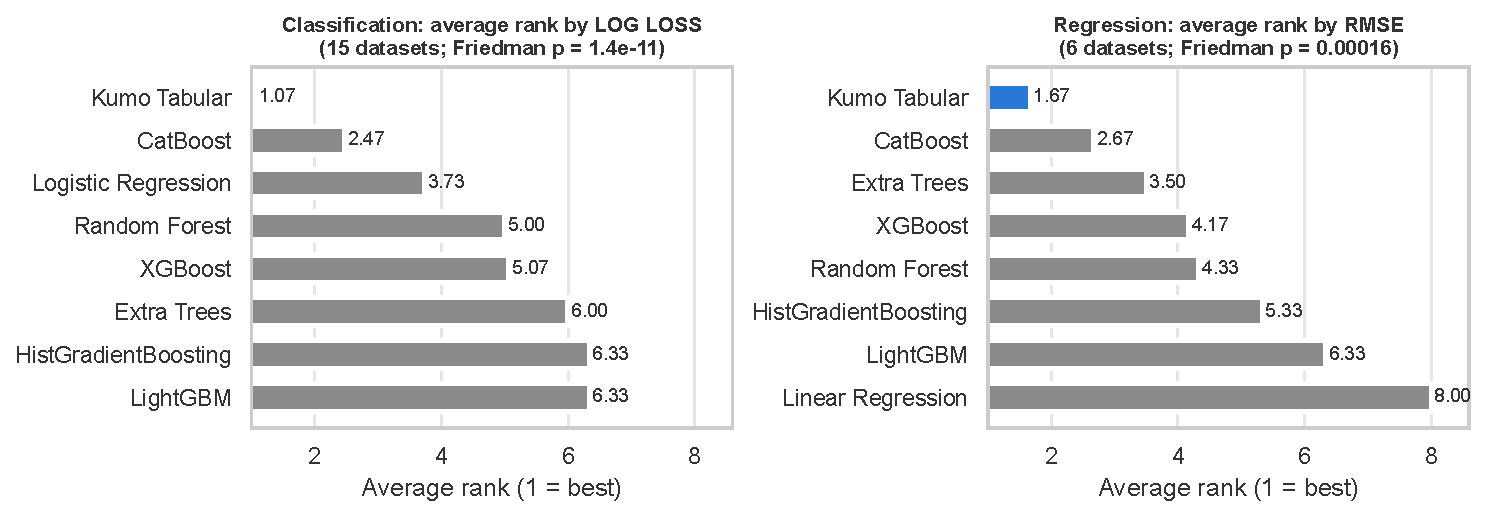
\includegraphics[width=\textwidth]{figures/average_ranks.pdf}
\caption{Average rank of each model on the primary metric across datasets (1 = best). Kumo Tabular in blue.}
\label{fig:ranks}
\end{figure}

\subsection{Regression}
On RMSE, Kumo Tabular had the best average rank (1.67; Friedman $p<0.001$), followed by CatBoost (2.67) and extra
trees (3.50); ordinary least squares ranked last on every dataset. Kumo Tabular had a lower RMSE than histogram gradient
boosting, LightGBM and least squares on all six datasets and than the other four baselines on five of six. None of these
differences is significant after Holm's correction (smallest adjusted $p=0.22$), as anticipated by the design: with six
datasets these comparisons cannot reach significance, and we treat them as descriptive. Relative to the best baseline on
each dataset, Kumo Tabular had a lower RMSE on four of six datasets, with the largest reduction on
\texttt{airfoil\_self\_noise} (44\%). It was clearly worse on \texttt{energy\_efficiency}, where its RMSE was 44\% higher
than XGBoost's, and slightly worse on \texttt{red\_wine} (5\% higher than extra trees). The secondary metrics MAE and
$R^2$ gave the same ordering of Kumo Tabular first (average ranks 1.33 and 1.67).

\begin{figure}[t]
\centering
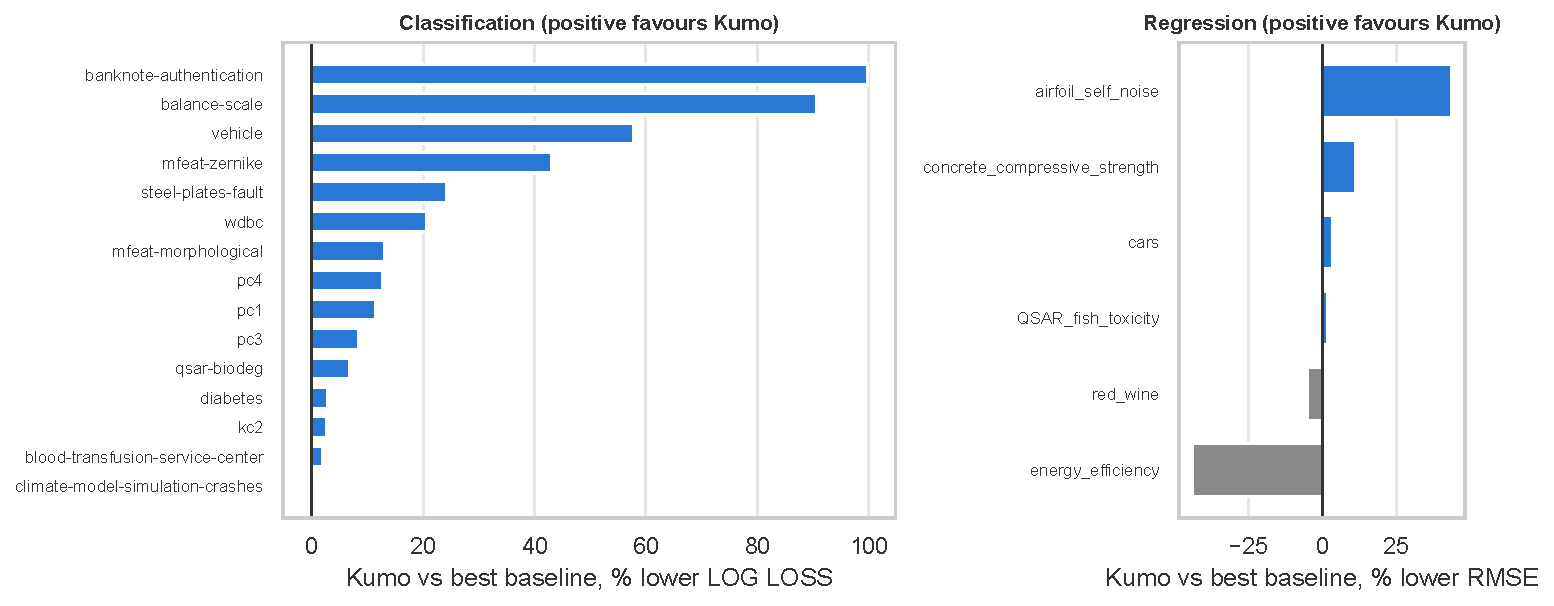
\includegraphics[width=\textwidth]{figures/per_dataset_primary_metric.pdf}
\caption{Per-dataset difference between Kumo Tabular and the best of the seven baselines on that dataset, as a
percentage of the baseline's loss (log loss for classification, RMSE for regression). Positive values favour Kumo
Tabular. Comparing against the per-dataset best baseline is stricter than any single fixed baseline.}
\label{fig:perdataset}
\end{figure}

\subsection{Sensitivity analyses}
The classification conclusions did not change in either planned sensitivity analysis (Table~\ref{tab:sensitivity}).
Without \texttt{wdbc}, Kumo Tabular's average rank was 1.07 and it was significantly better than all seven baselines
after Holm's correction; with related datasets averaged into single units (11 units), its average rank was 1.09 and all
seven comparisons remained significant (adjusted $p=0.007$). The regression results were unchanged because no
regression dataset was affected.

\begin{table}[t]
\centering
\small
\caption{Planned sensitivity analyses on the primary metric: Kumo Tabular's average rank, the number of baselines it beats with Holm-adjusted $p<0.05$, and its W/T/L against the strongest baseline (lowest average rank).}
\label{tab:sensitivity}
\begin{tabular}{llcccc}
\toprule
Task & Analysis & $n$ & Kumo avg.\ rank & Sig.\ wins (of 7) & W/T/L vs strongest \\
\midrule
Classification & All datasets & 15 & 1.07 & 7 & 15/0/0 (CatBoost) \\
 & Excluding wdbc & 14 & 1.07 & 7 & 14/0/0 (CatBoost) \\
 & Families collapsed & 11 & 1.09 & 7 & 11/0/0 (CatBoost) \\
\midrule
Regression & All datasets & 6 & 1.67 & 0 & 5/0/1 (CatBoost) \\
 & Excluding wdbc & 6 & 1.67 & 0 & 5/0/1 (CatBoost) \\
 & Families collapsed & 6 & 1.67 & 0 & 5/0/1 (CatBoost) \\
\bottomrule
\end{tabular}
\end{table}


\subsection{Runtime}
Table~\ref{tab:runtime} and Figure~\ref{fig:runtime} report fit-plus-prediction time per fold. On this hardware the
median time per fold of Kumo Tabular on the GPU (1.27\,s for classification, 1.14\,s for regression) was comparable to
500-tree random forests and extra trees on the CPU and lower than CatBoost with its default 1{,}000 iterations. It was
about 7 (classification) and 9 to 11 (regression) times the median time of XGBoost and LightGBM, and about 48 times
that of logistic regression and 300 times that of least squares. The time per fold depended strongly on
the dataset: on the 10-class \texttt{mfeat-zernike} dataset the ten folds took 1{,}113\,s for histogram gradient
boosting, 841\,s for CatBoost and 650\,s for Kumo Tabular, against 21\,s or less for XGBoost, LightGBM, extra trees and
logistic regression. These measurements are hardware-specific (Section~\ref{sec:limitations}).

\begin{table}[t]
\centering
\small
\caption{Fit plus prediction time per fold in seconds: median [interquartile range] over all folds of all datasets. Kumo Tabular ran on an NVIDIA GTX 980M GPU (float32); all other models on an Intel Core i7-6700HQ CPU. Times are hardware-dependent and not comparable as algorithmic costs.}
\label{tab:runtime}
\begin{tabular}{lll}
\toprule
Model & Classification & Regression \\
\midrule
Kumo Tabular & 1.275 [0.896, 3.053] & 1.142 [0.929, 1.471] \\
Logistic reg. & 0.027 [0.015, 0.053] & -- \\
Linear reg. & -- & 0.004 [0.003, 0.005] \\
Random forest & 1.392 [1.284, 1.542] & 1.077 [1.038, 1.165] \\
Extra trees & 1.087 [1.001, 1.242] & 0.753 [0.737, 0.789] \\
HistGB & 0.487 [0.323, 1.474] & 0.379 [0.341, 0.403] \\
XGBoost & 0.181 [0.114, 0.283] & 0.125 [0.110, 0.152] \\
LightGBM & 0.168 [0.094, 0.318] & 0.103 [0.092, 0.117] \\
CatBoost & 4.564 [3.251, 5.824] & 1.728 [1.348, 2.018] \\
\bottomrule
\end{tabular}
\end{table}


\begin{figure}[t]
\centering
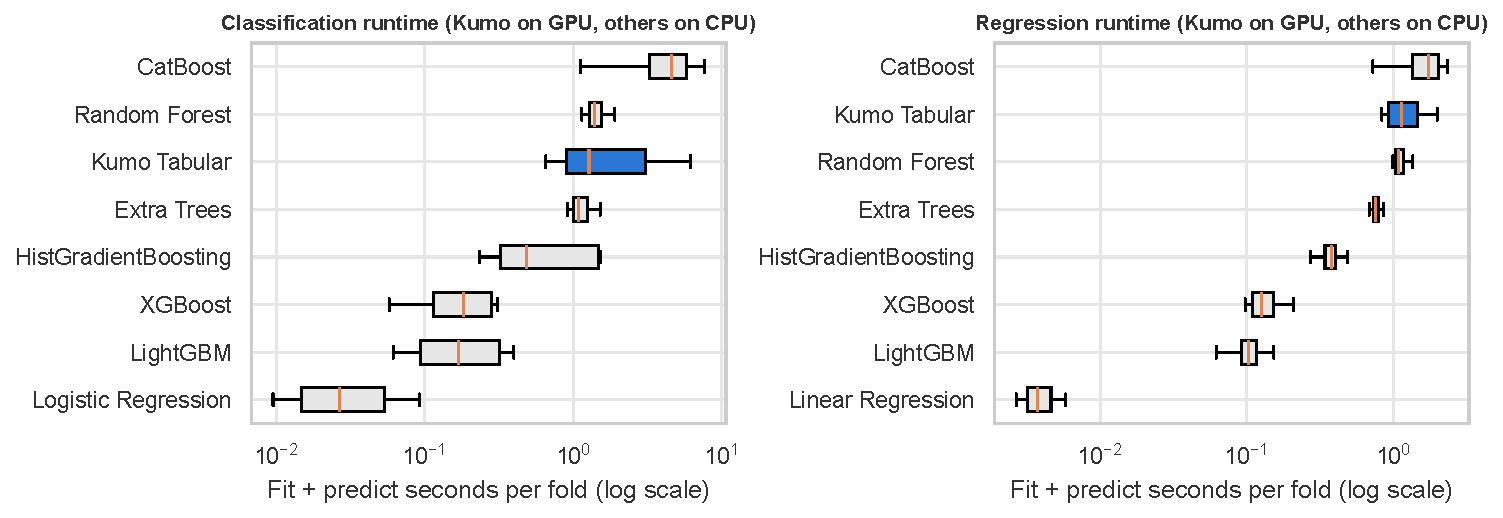
\includegraphics[width=\textwidth]{figures/runtime.pdf}
\caption{Fit plus prediction time per fold (log scale) over all folds of all datasets. Kumo Tabular ran on a GPU, the
other models on a CPU.}
\label{fig:runtime}
\end{figure}

\subsection{Case studies}
\label{sec:case}
The two-dataset case studies (Appendix~\ref{app:case}) are consistent with the benchmark but add detail. On breast
cancer data Kumo Tabular had the best mean on every threshold metric (accuracy 0.989 versus 0.977 for logistic
regression) and higher accuracy than logistic regression on all five splits, but after the overlap correction and Holm's
adjustment no within-dataset comparison was significant (smallest adjusted $p=0.081$). On diabetes data it was
indistinguishable from linear regression ($R^2$ 0.503 versus 0.496). In the training-size study it was much more robust
than least squares with 25 training rows ($R^2$ 0.429 versus 0.075) but no better than logistic regression for
classification at 25 to 100 rows. Its nominal 90\% quantile interval covered 93.3\% of diabetes test targets.

\section{Discussion}
\label{sec:discussion}

\paragraph{What the evidence establishes.}
On 15 small, fully numerical classification datasets, the \texttt{small} Kumo Tabular checkpoint with default settings
produced better probabilistic predictions than each of seven untuned classical models, consistently across datasets,
with differences that survive multiplicity correction and both sensitivity analyses (RQ1, RQ2). The advantage also
appears in ROC-AUC, so it is not explained by calibration alone. On six regression datasets it ranked first on average,
but the evidence is too limited for a statistical claim.

\paragraph{Where it does not help.}
The aggregate hides dataset-level exceptions (RQ3). Kumo Tabular's accuracy was below the best baseline on three of 15
classification datasets, and its RMSE was 44\% higher than XGBoost's on \texttt{energy\_efficiency}. In the case
studies, logistic regression matched it for classification with 25 to 100 training rows, and on the diabetes data
linear regression was statistically indistinguishable from it. The largest accuracy gains occurred on two multiclass
datasets (\texttt{vehicle}, \texttt{balance-scale}); on several binary tasks the differences in accuracy were a fraction
of a percentage point.

\paragraph{Interpreting the comparison.}
The baselines were not tuned, whereas Kumo Tabular's defaults result from extensive pretraining. Our comparison
therefore answers a practical question---what a practitioner obtains without model selection on small numerical
tables---and not which model class is better when each is tuned. Regularized or tuned gradient boosting, and a strong
linear model for nearly linear targets, remain relevant alternatives.

\paragraph{Cost.}
Prediction with Kumo Tabular processes the full context at every call. On our hardware its time per fold was comparable
to large random forests and smaller than CatBoost's, but well above linear models, XGBoost and LightGBM, and it requires
a GPU for reasonable speed (RQ4).

\section{Conclusion}
\label{sec:conclusion}
In an independent evaluation on 21 small numerical OpenML datasets, the smallest Kumo Tabular checkpoint
outperformed seven untuned classical baselines on classification log loss on nearly every dataset, and ranked first on
average for regression without statistical support. The results justify Kumo Tabular as a strong default for small
numerical tables, while the dataset-level exceptions, the restricted data regime and the untuned baselines limit how
far the conclusion extends.

\section{Limitations and Threats to Validity}
\label{sec:limitations}

\paragraph{Scope of the datasets.}
All datasets are small (at most 2{,}000 rows), fully numerical and complete. Our conclusions do not extend to larger
tables, categorical or text features, or missing values---settings that tabular foundation models are designed to
handle and in which their relative performance may differ. The datasets come from two curated suites; curation and the
selection filters shape which problems are represented. The filters relied on OpenML metadata, which was wrong for
\texttt{forest\_fires}: it was excluded at load time because of undeclared text columns, after results for 17 other
datasets existed. The exclusion follows the selection criterion and did not depend on any result, but it reduced the
regression suite from seven to six datasets, and we did not evaluate the dataset with its text columns encoded or
removed. Six regression datasets support descriptive conclusions only.

\paragraph{Dependence between datasets.}
Some datasets share a source (four NASA software-defect datasets; two \texttt{mfeat} feature sets of the same digits),
which violates the independence assumed by the Friedman and Wilcoxon tests. The planned family-collapsed analysis
addresses this only partly.

\paragraph{Untuned baselines and a single checkpoint.}
No model was tuned. Tuned gradient boosting or regularized linear models could narrow or reverse differences, and
library defaults are not designed for very small data. Only the \texttt{small} Kumo Tabular checkpoint was evaluated,
with float32 inference on an older GPU; the developers' claims concern larger checkpoints as well.

\paragraph{Pretraining overlap.}
The developers state that Kumo Tabular was pretrained on synthetic data only \citep{nvidia_kumo_blog}. We cannot verify
this; if any benchmark dataset or close variant was seen in pretraining, Kumo Tabular's performance on it would be
overstated.

\paragraph{Statistical power and multiplicity.}
With 15 classification datasets the cross-dataset tests can detect only consistent differences; absence of
significance is not evidence of equivalence. Secondary metrics and sensitivity analyses are not adjusted for
multiplicity and are descriptive. Within-dataset comparisons in the case studies rest on five dependent splits.

\paragraph{Timing of the analysis plan.}
The analysis plan was written after the complete results on \texttt{wdbc} had been seen, on which Kumo Tabular was best
on all quality metrics, and it is timestamped only in a local repository. Choices made in the plan, such as the
primary metrics, could in principle have been influenced by that one dataset. The analysis without \texttt{wdbc}
gives the same conclusions (Table~\ref{tab:sensitivity}), and the secondary metrics are reported in full.

\paragraph{Runtime.}
Runtimes come from one laptop with a GPU for Kumo Tabular and a CPU for all other models, and timings of a few
milliseconds vary between runs. They indicate orders of magnitude on this hardware, not algorithmic costs.

\paragraph{Construct validity.}
Accuracy and macro-F1 use the arg-max decision rule; in applications the decision threshold would be chosen for a
target cost. The medical case-study datasets are used as benchmarks only; no conclusion about clinical use is drawn.


\section*{Reproducibility Statement}
The anonymized supplementary material \citep{anonymous2026supplement} contains all code, the dataset selection script and its output, raw per-fold
and per-split results, run logs, environment records, the analysis plan and the analysis and validation scripts. The
datasets and splits are public on OpenML; the model weights are public on Hugging Face. All 45 unit tests pass,
including tests for data leakage and prediction shapes. The OpenML benchmark ran for about 1.5 hours on the hardware in
Appendix~\ref{app:software}.

\section*{Broader Impact Statement}
This is a benchmark study of an existing, publicly released model on public datasets. We do not foresee a significant
risk of harm. Two case-study datasets are medical; they are used only as benchmarks, and our results must not be read
as evidence about clinical use.

\bibliography{references}
\bibliographystyle{tmlr}

\appendix

\section{Per-Dataset Results of the Main Benchmark}
\label{app:perdataset}

Tables~\ref{tab:perdataset_classification} and~\ref{tab:perdataset_regression} give the primary metric for every model
and dataset (mean over 10 folds). All per-fold results, including the secondary metrics and timings, are in the
supplementary material.

\begin{table}[h]
\centering
\scriptsize
\setlength{\tabcolsep}{3pt}
\caption{Per-dataset log loss (classification), mean over 10 folds. Best value per dataset in bold.}
\label{tab:perdataset_classification}
\smallskip
\begin{adjustbox}{max width=\textwidth}
\begin{tabular}{lrrrrrrrr}
\toprule
Dataset & Kumo Tabular & Logistic reg. & Random forest & Extra trees & HistGB & XGBoost & LightGBM & CatBoost \\
\midrule
balance-scale & \textbf{0.024} & 0.278 & 0.535 & 2.853 & 0.407 & 0.319 & 0.331 & 0.255 \\
banknote-authentication & \textbf{0.000} & 0.048 & 0.027 & 0.014 & 0.015 & 0.015 & 0.023 & 0.008 \\
blood-transfusion-service-center & \textbf{0.468} & 0.477 & 0.782 & 2.490 & 0.579 & 0.609 & 0.559 & 0.490 \\
climate-model-simulation-crashes & 0.131 & \textbf{0.131} & 0.190 & 0.183 & 0.182 & 0.149 & 0.198 & 0.140 \\
diabetes & \textbf{0.466} & 0.485 & 0.480 & 0.483 & 0.632 & 0.721 & 0.628 & 0.480 \\
kc2 & \textbf{0.374} & 0.386 & 0.754 & 0.821 & 0.515 & 0.531 & 0.526 & 0.384 \\
mfeat-morphological & \textbf{0.559} & 0.643 & 0.944 & 4.116 & 1.143 & 0.887 & 1.126 & 0.648 \\
mfeat-zernike & \textbf{0.213} & 0.374 & 0.687 & 3.743 & 0.967 & 0.724 & 0.938 & 0.541 \\
pc1 & \textbf{0.160} & 0.227 & 0.181 & 0.545 & 0.297 & 0.240 & 0.315 & 0.180 \\
pc3 & \textbf{0.236} & 0.283 & 0.265 & 0.332 & 0.357 & 0.353 & 0.355 & 0.258 \\
pc4 & \textbf{0.157} & 0.229 & 0.197 & 0.224 & 0.236 & 0.223 & 0.226 & 0.180 \\
qsar-biodeg & \textbf{0.284} & 0.334 & 0.341 & 0.368 & 0.381 & 0.376 & 0.409 & 0.305 \\
steel-plates-fault & \textbf{0.383} & 0.773 & 0.577 & 0.573 & 0.669 & 0.568 & 0.647 & 0.506 \\
vehicle & \textbf{0.199} & 0.472 & 0.498 & 0.517 & 0.697 & 0.579 & 0.613 & 0.475 \\
wdbc & \textbf{0.062} & 0.078 & 0.112 & 0.108 & 0.110 & 0.091 & 0.119 & 0.082 \\
\bottomrule
\end{tabular}
\end{adjustbox}
\end{table}


\begin{table}[h]
\centering
\scriptsize
\setlength{\tabcolsep}{3pt}
\caption{Per-dataset RMSE (regression), mean over 10 folds. Best value per dataset in bold.}
\label{tab:perdataset_regression}
\smallskip
\begin{adjustbox}{max width=\textwidth}
\begin{tabular}{lrrrrrrrr}
\toprule
Dataset & Kumo Tabular & Linear reg. & Random forest & Extra trees & HistGB & XGBoost & LightGBM & CatBoost \\
\midrule
QSAR\_fish\_toxicity & \textbf{0.841} & 0.954 & 0.884 & 0.882 & 0.897 & 0.944 & 0.899 & 0.857 \\
airfoil\_self\_noise & \textbf{0.780} & 4.823 & 1.648 & 1.390 & 1.789 & 1.462 & 1.790 & 1.466 \\
cars & \textbf{2037.702} & 2944.899 & 2307.586 & 2418.453 & 2481.138 & 2389.355 & 2484.833 & 2111.137 \\
concrete\_compressive\_strength & \textbf{3.490} & 10.436 & 4.777 & 4.509 & 4.376 & 4.148 & 4.406 & 3.928 \\
energy\_efficiency & 0.416 & 2.943 & 0.449 & 0.438 & 0.482 & \textbf{0.289} & 0.482 & 0.291 \\
red\_wine & 0.570 & 0.651 & 0.559 & \textbf{0.543} & 0.586 & 0.595 & 0.587 & 0.573 \\
\bottomrule
\end{tabular}
\end{adjustbox}
\end{table}


\section{Case Studies: Breast Cancer and Diabetes}
\label{app:case}

The case studies use five stratified (classification) or random (regression) 80/20 splits with seeds 42--46, logistic
or linear regression, random forests (500 trees) and histogram gradient boosting with defaults, and Kumo Tabular with
the same settings as the main benchmark. Malignant tumours are the positive class. Tables~\ref{tab:classification}
and~\ref{tab:regression} report means and standard deviations over the splits; Table~\ref{tab:paired} the
within-dataset paired comparison with the strongest baseline; Tables~\ref{tab:study_classification}
and~\ref{tab:study_regression} the training-size study (seeds 42--44); and Figure~\ref{fig:case} the training-size
curves and Kumo Tabular's quantile intervals. Because five resampled splits are dependent, these analyses are
descriptive; no within-dataset difference is significant after the overlap correction and Holm's adjustment. A
complete re-run of the same code reproduced all metrics exactly, and execution of the same notebooks in a separate
cloud environment (NVIDIA T4, PyTorch 2.11,
float16) reproduced the results of Kumo Tabular, logistic/linear regression and random forests at the reported
precision; histogram gradient boosting differed slightly there (for example, accuracy 0.960 instead of 0.967).

\begin{table*}[t]
\centering
\caption{Breast cancer classification results (mean $\pm$ standard deviation over five stratified splits, 114 test rows each). Malignant is the positive class. Time is fit plus prediction time per split. Best mean per metric in bold.}
\label{tab:classification}
\setlength{\tabcolsep}{5pt}
\smallskip
\begin{adjustbox}{max width=\textwidth}
\begin{tabular}{lcccccc}
\toprule
Model & Accuracy & Precision & Recall & F1 & ROC-AUC & Time (s) \\
\midrule
Kumo Tabular & \textbf{0.989 $\pm$ 0.010} & \textbf{0.995 $\pm$ 0.010} & \textbf{0.976 $\pm$ 0.029} & \textbf{0.985 $\pm$ 0.014} & \textbf{0.998 $\pm$ 0.003} & 1.099 $\pm$ 0.012 \\
Logistic Reg. & 0.977 $\pm$ 0.012 & 0.990 $\pm$ 0.013 & 0.948 $\pm$ 0.031 & 0.968 $\pm$ 0.017 & 0.995 $\pm$ 0.004 & 0.019 $\pm$ 0.001 \\
Random Forest & 0.954 $\pm$ 0.013 & 0.947 $\pm$ 0.031 & 0.929 $\pm$ 0.024 & 0.938 $\pm$ 0.018 & 0.988 $\pm$ 0.011 & 1.204 $\pm$ 0.063 \\
HistGB & 0.967 $\pm$ 0.016 & 0.976 $\pm$ 0.024 & 0.933 $\pm$ 0.043 & 0.953 $\pm$ 0.022 & 0.994 $\pm$ 0.007 & 0.274 $\pm$ 0.020 \\
\bottomrule
\end{tabular}
\end{adjustbox}
\end{table*}


\begin{table*}[t]
\centering
\caption{Diabetes regression results (mean $\pm$ standard deviation over five random splits, 89 test rows each). Kumo Tabular uses the median quantile $q_{0.5}$ as point prediction. Best mean per metric in bold.}
\label{tab:regression}
\setlength{\tabcolsep}{5pt}
\smallskip
\begin{adjustbox}{max width=\textwidth}
\begin{tabular}{lcccc}
\toprule
Model & MAE & RMSE & $R^2$ & Time (s) \\
\midrule
Kumo Tabular & \textbf{42.48 $\pm$ 3.10} & \textbf{52.88 $\pm$ 3.47} & \textbf{0.503 $\pm$ 0.039} & 0.627 $\pm$ 0.053 \\
Linear Reg. & 43.75 $\pm$ 3.59 & 53.27 $\pm$ 4.03 & 0.496 $\pm$ 0.046 & 0.003 $\pm$ 0.000 \\
Random Forest & 45.23 $\pm$ 2.63 & 56.16 $\pm$ 3.31 & 0.440 $\pm$ 0.022 & 0.833 $\pm$ 0.024 \\
HistGB & 45.85 $\pm$ 0.72 & 58.52 $\pm$ 1.67 & 0.390 $\pm$ 0.042 & 0.190 $\pm$ 0.031 \\
\bottomrule
\end{tabular}
\end{adjustbox}
\end{table*}


\begin{table*}[t]
\centering
\caption{Paired comparison of Kumo Tabular with the strongest baseline over the five splits. $\overline{d}$ is the mean advantage of Kumo (positive favours Kumo for every metric), $s_d$ its standard deviation. The corrected test and interval use the Nadeau--Bengio variance correction for overlapping training sets; Holm adjustment is applied within each task. No result is significant at $\alpha=0.05$ after adjustment.}
\label{tab:paired}
\setlength{\tabcolsep}{4.5pt}
\smallskip
\begin{adjustbox}{max width=\textwidth}
\begin{tabular}{llcccccccc}
\toprule
Task & Metric & W/T/L & $\overline{d}$ & $s_d$ & Corrected 95\% CI & $p_{\mathrm{naive}}$ & $p_{\mathrm{corr}}$ & $p_{\mathrm{corr}}^{\mathrm{Holm}}$ & $p_{\mathrm{Wilcoxon}}$ \\
\midrule
Classification & Accuracy & 5/0/0 & 0.0123 & 0.0078 & [$-$0.0023, 0.0269] & 0.025 & 0.080 & 0.313 & 0.062 ($n$=5) \\
 & Precision & 2/3/0 & 0.0051 & 0.0111 & [$-$0.0156, 0.0258] & 0.362 & 0.531 & 0.535 & 0.500 ($n$=2) \\
 & Recall & 5/0/0 & 0.0286 & 0.0106 & [0.0087, 0.0484] & 0.004 & 0.016 & 0.081 & 0.062 ($n$=5) \\
 & F1 & 5/0/0 & 0.0172 & 0.0109 & [$-$0.0031, 0.0376] & 0.024 & 0.078 & 0.313 & 0.062 ($n$=5) \\
 & ROC-AUC & 4/1/0 & 0.0030 & 0.0034 & [$-$0.0034, 0.0094] & 0.126 & 0.267 & 0.535 & 0.125 ($n$=4) \\
\midrule
Regression & MAE & 4/0/1 & 1.27 & 1.10 & [$-$0.78, 3.32] & 0.061 & 0.161 & 0.484 & 0.125 ($n$=5) \\
 & RMSE & 3/0/2 & 0.39 & 1.43 & [$-$2.28, 3.07] & 0.573 & 0.704 & 1.000 & 0.625 ($n$=5) \\
 & $R^2$ & 3/0/2 & 0.007 & 0.028 & [$-$0.046, 0.060] & 0.603 & 0.727 & 1.000 & 0.625 ($n$=5) \\
\bottomrule
\end{tabular}
\end{adjustbox}
\end{table*}


\begin{table}[t]
\centering
\caption{Classification accuracy by training-set size (mean $\pm$ standard deviation over three seeds; full test split).}
\label{tab:study_classification}
\setlength{\tabcolsep}{3pt}
\begin{tabular}{rcccc}
\toprule
$n$ & Kumo Tabular & Logistic Reg. & Random Forest & HistGB \\
\midrule
25 & 0.950\,{\scriptsize$\pm$0.027} & \textbf{0.956}\,{\scriptsize$\pm$0.023} & 0.930\,{\scriptsize$\pm$0.018} & 0.632\,{\scriptsize$\pm$0.000} \\
50 & \textbf{0.953}\,{\scriptsize$\pm$0.051} & \textbf{0.953}\,{\scriptsize$\pm$0.022} & 0.933\,{\scriptsize$\pm$0.044} & 0.909\,{\scriptsize$\pm$0.035} \\
100 & \textbf{0.956}\,{\scriptsize$\pm$0.040} & \textbf{0.956}\,{\scriptsize$\pm$0.026} & 0.939\,{\scriptsize$\pm$0.015} & 0.944\,{\scriptsize$\pm$0.051} \\
200 & \textbf{0.985}\,{\scriptsize$\pm$0.013} & 0.971\,{\scriptsize$\pm$0.013} & 0.947\,{\scriptsize$\pm$0.009} & 0.947\,{\scriptsize$\pm$0.009} \\
400 & \textbf{0.982}\,{\scriptsize$\pm$0.015} & 0.974\,{\scriptsize$\pm$0.015} & 0.953\,{\scriptsize$\pm$0.018} & 0.956\,{\scriptsize$\pm$0.009} \\
455 & \textbf{0.988}\,{\scriptsize$\pm$0.013} & 0.974\,{\scriptsize$\pm$0.015} & 0.959\,{\scriptsize$\pm$0.013} & 0.959\,{\scriptsize$\pm$0.010} \\
\bottomrule
\end{tabular}
\end{table}


\begin{table}[t]
\centering
\caption{Regression $R^2$ by training-set size (mean $\pm$ standard deviation over three seeds; full test split).}
\label{tab:study_regression}
\setlength{\tabcolsep}{3pt}
\begin{tabular}{rcccc}
\toprule
$n$ & Kumo Tabular & Linear Reg. & Random Forest & HistGB \\
\midrule
25 & \textbf{0.429}\,{\scriptsize$\pm$0.058} & 0.075\,{\scriptsize$\pm$0.304} & 0.388\,{\scriptsize$\pm$0.127} & $-$0.097\,{\scriptsize$\pm$0.087} \\
50 & \textbf{0.437}\,{\scriptsize$\pm$0.019} & 0.331\,{\scriptsize$\pm$0.137} & 0.418\,{\scriptsize$\pm$0.008} & 0.348\,{\scriptsize$\pm$0.063} \\
100 & \textbf{0.486}\,{\scriptsize$\pm$0.045} & 0.467\,{\scriptsize$\pm$0.076} & 0.433\,{\scriptsize$\pm$0.024} & 0.410\,{\scriptsize$\pm$0.043} \\
200 & 0.505\,{\scriptsize$\pm$0.085} & \textbf{0.506}\,{\scriptsize$\pm$0.060} & 0.438\,{\scriptsize$\pm$0.057} & 0.391\,{\scriptsize$\pm$0.069} \\
353 & \textbf{0.526}\,{\scriptsize$\pm$0.028} & 0.507\,{\scriptsize$\pm$0.048} & 0.440\,{\scriptsize$\pm$0.024} & 0.406\,{\scriptsize$\pm$0.030} \\
\bottomrule
\end{tabular}
\end{table}


\begin{figure}[h]
\centering
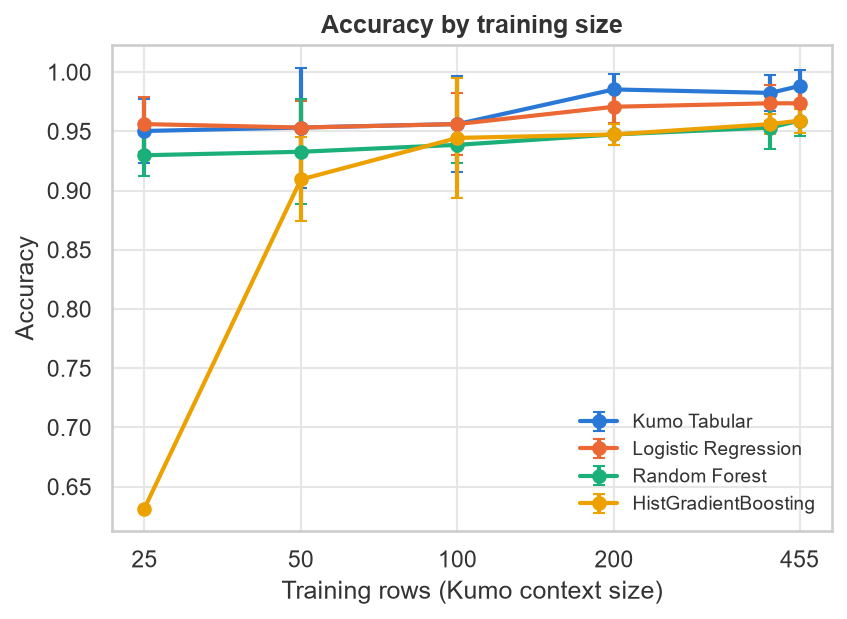
\includegraphics[width=0.32\textwidth]{figures/original_classification_sample_size_accuracy.png}\hfill
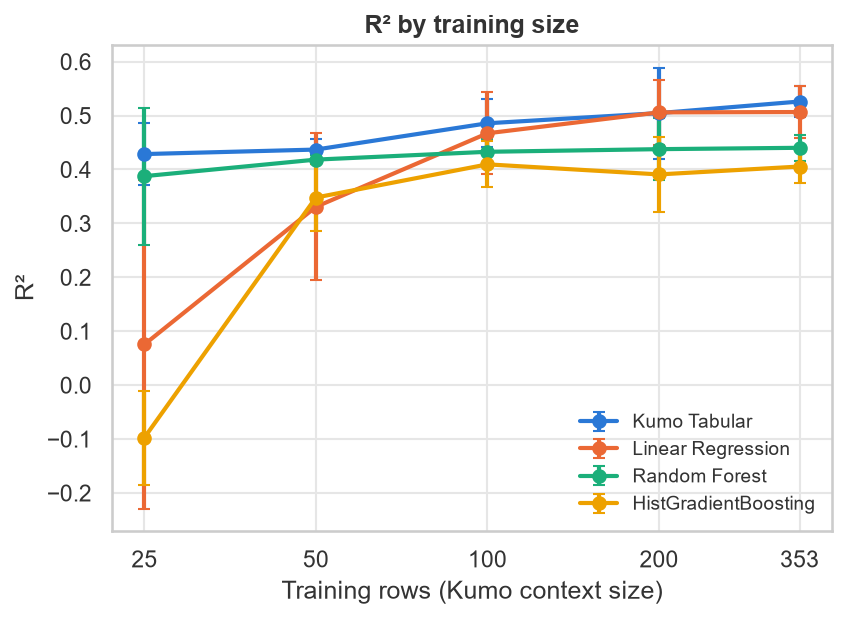
\includegraphics[width=0.32\textwidth]{figures/original_regression_sample_size_r2.png}\hfill
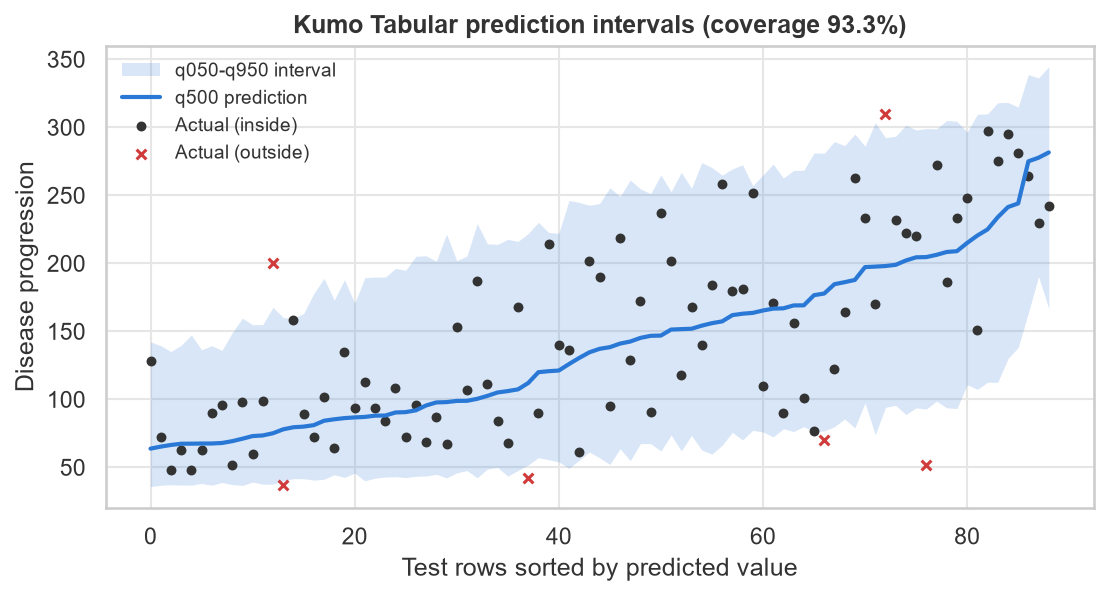
\includegraphics[width=0.32\textwidth]{figures/original_regression_kumo_intervals.png}
\caption{Case studies: classification accuracy and regression $R^2$ by number of training rows (mean $\pm$ one standard
deviation over three seeds; logarithmic horizontal axis), and Kumo Tabular's median prediction with its nominal 90\%
interval on one diabetes split (coverage 93.3\% on that split).}
\label{fig:case}
\end{figure}

\section{Software and Hardware}
\label{app:software}

Python 3.12.16, PyTorch 2.14.1 \citep{paszke2019pytorch} (CUDA 12.6), structured-data-models 0.2.1, scikit-learn 1.9.1, XGBoost 3.4.1, LightGBM
4.7.0, CatBoost 1.2.10, NumPy 2.5.4, pandas 3.1.0; NVIDIA GeForce GTX 980M (8\,GB, compute capability 5.2), Intel Core
i7-6700HQ, 16\,GB RAM, Windows 10. Kumo Tabular weights: Hugging Face repository \texttt{nvidia/Kumo-Tabular}, revision
\texttt{v1.0.1}, \texttt{small} checkpoints.


\end{document}
